\section{物理モデル}
    本章ではまず結合共振回路の物理モデルの説明から始める。
\section{超伝導回路素子}
    サンプル作成に使用した超伝導回路素子の説明を包括的に行う。まずは超伝導共振器の導入を行う。
    \subsection{超伝導共振器}
    超伝導共振素子は量子コンピュータ\cite*{Goppl2008}や量子増幅器、光子メモリ\cite*{Pierre2014}、そして結合素子\cite*{Baust2015,Reuther2009}等様々なデバイスに応用されている。
        この章では超伝導体を用いた共振素子についてマイクロ波エンジニアリングに基づいて記述する。\cite*{Microwave}
        最も簡便な共振モデルは図のようなLC共振回路である。
        \begin{figure}[H]
            \centering
            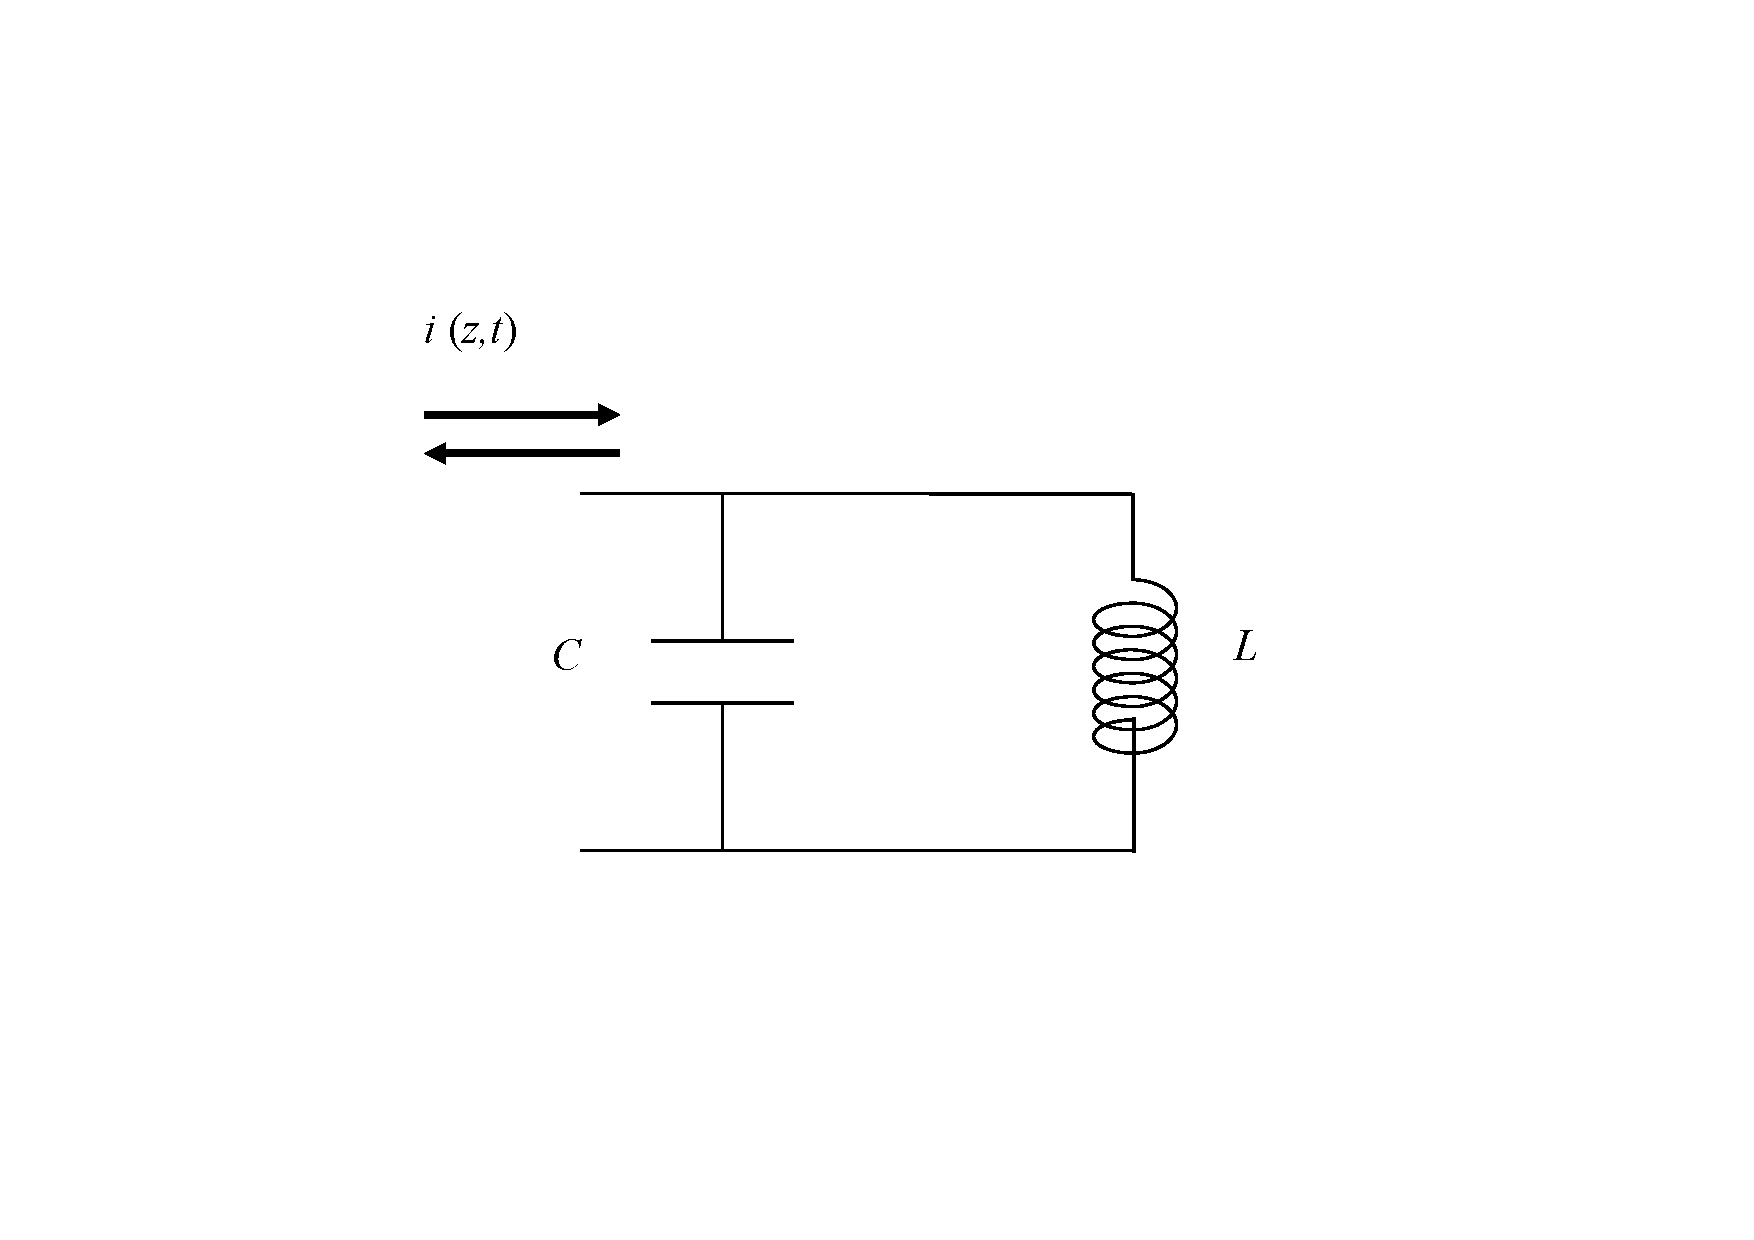
\includegraphics[width=9cm]{le.pdf}
            \caption{エネルギースペクトル}
        \end{figure}
        このとき共振周波数は回路のインダクタンスとキャパシタンスを用いて$\omega_0=1/\sqrt{LC}$と表現できる。
        図のような平行共振回路の複素インピーダンスは
        \begin{equation}
            Z_{i n}=\frac{1}{\frac{1}{R}+\frac{1}{j \omega L}+j \omega C}
        \end{equation}
        のように記述できる。この時共振回路のパワーはオームの法則により
        \begin{equation}
            P_{i n}=\frac{1}{2} V I^{*}=\frac{1}{2}|V|^{2}\left(\frac{1}{R}+\frac{j}{\omega L}-j \omega C\right)
            \end{equation}
        と表現することができる。LC共振回路において抵抗は損失である。損失分のパワーは
        \begin{equation}
            P_{\text {loss }}=\frac{1}{2} \frac{|V|^{2}}{R}
        \end{equation}
        と表現される。また、共振回路中キャパシタンス及びインダクタンスに蓄えられる平均エネルギーはそれぞれ
        \begin{equation}
            \begin{array}{l}
            W_{m}=\frac{1}{4}|V|^{2} \frac{1}{\omega^{2} L} \\
            W_{e}=\frac{1}{4}|V|^{2} \frac{1}{\omega^{2} L} .
            \end{array}
            \end{equation}
        と記述することができる。共振器の性能を表す特徴量であるQ値は損失に対して蓄えられるエネルギー量の指標であり、次のように表現される。
        \begin{equation}
            Q_{\text {int }}=\omega \frac{共振回路の平均エネルギー}{単位時間あたりの損失エネルギー}
        \end{equation}
        上記の式を代入することで
        \begin{equation}
            Q_{\text {int }}=\omega \frac{W_{e}+W_{m}}{P_{\text {loss }}}=\omega_{0} \frac{2 W_{m}}{P_{\text {loss }}}=\frac{R}{\omega_{0} L}=\omega_{0} R C .
        \end{equation}
        のように記述できる。ここでQ値にintと添え字をつけたがこれは共振回路自身のQ値を表している。しかしながら回路としては共振回路に接続されることで生じるQ値も存在している。これを$Q_{ext}$と表現すると、回路全体のQ値は
        \begin{equation}
            \frac{1}{Q_{\text {total }}}=\frac{1}{Q_{\text {int }}}+\frac{1}{Q_{\text {ext }}}
        \end{equation}
        と表現される。

        ここで共振回路の観測可能量について説明をする。当研究室では共振器の測定にVNA(ベクトルネットワークアナライザ)を用いている。この測定機器はローカルオシレーターを内蔵しており、入力信号と反射信号そして透過信号を参照することにより被測定物の散乱パラメータを測定することができる。
        散乱パラメータは共振回路の共振周波数及びQ値を用いることにより、次のように表現できる。
        \begin{equation}
            S_{21}(f)=\frac{Q_{total} / Q_{ext}}{1+2 j Q_{total}\left(f-f_{0}\right) / f_{0}}
        \end{equation}
        また透過係数は
        \begin{equation}
            S_{11}(f)=1-\frac{Q_{m} / Q_{c}}{1+2 j Q_{m}\left(f-f_{0}\right) / f_{0}}
        \end{equation}
        である。測定では透過係数及び反射係数の絶対値を上記関数でフィットし、共振回路を評価する。

        次に超伝導共振器として特に利用される回路デザインとして超伝導分布定数回路及び超伝導準集中定数共振回路について記述する。
        \subsubsection{超伝導分布定数回路}
            最も使用頻度の高いデザインは平面型共振回路(CPW)である。
            \begin{figure}[H]
                \centering
                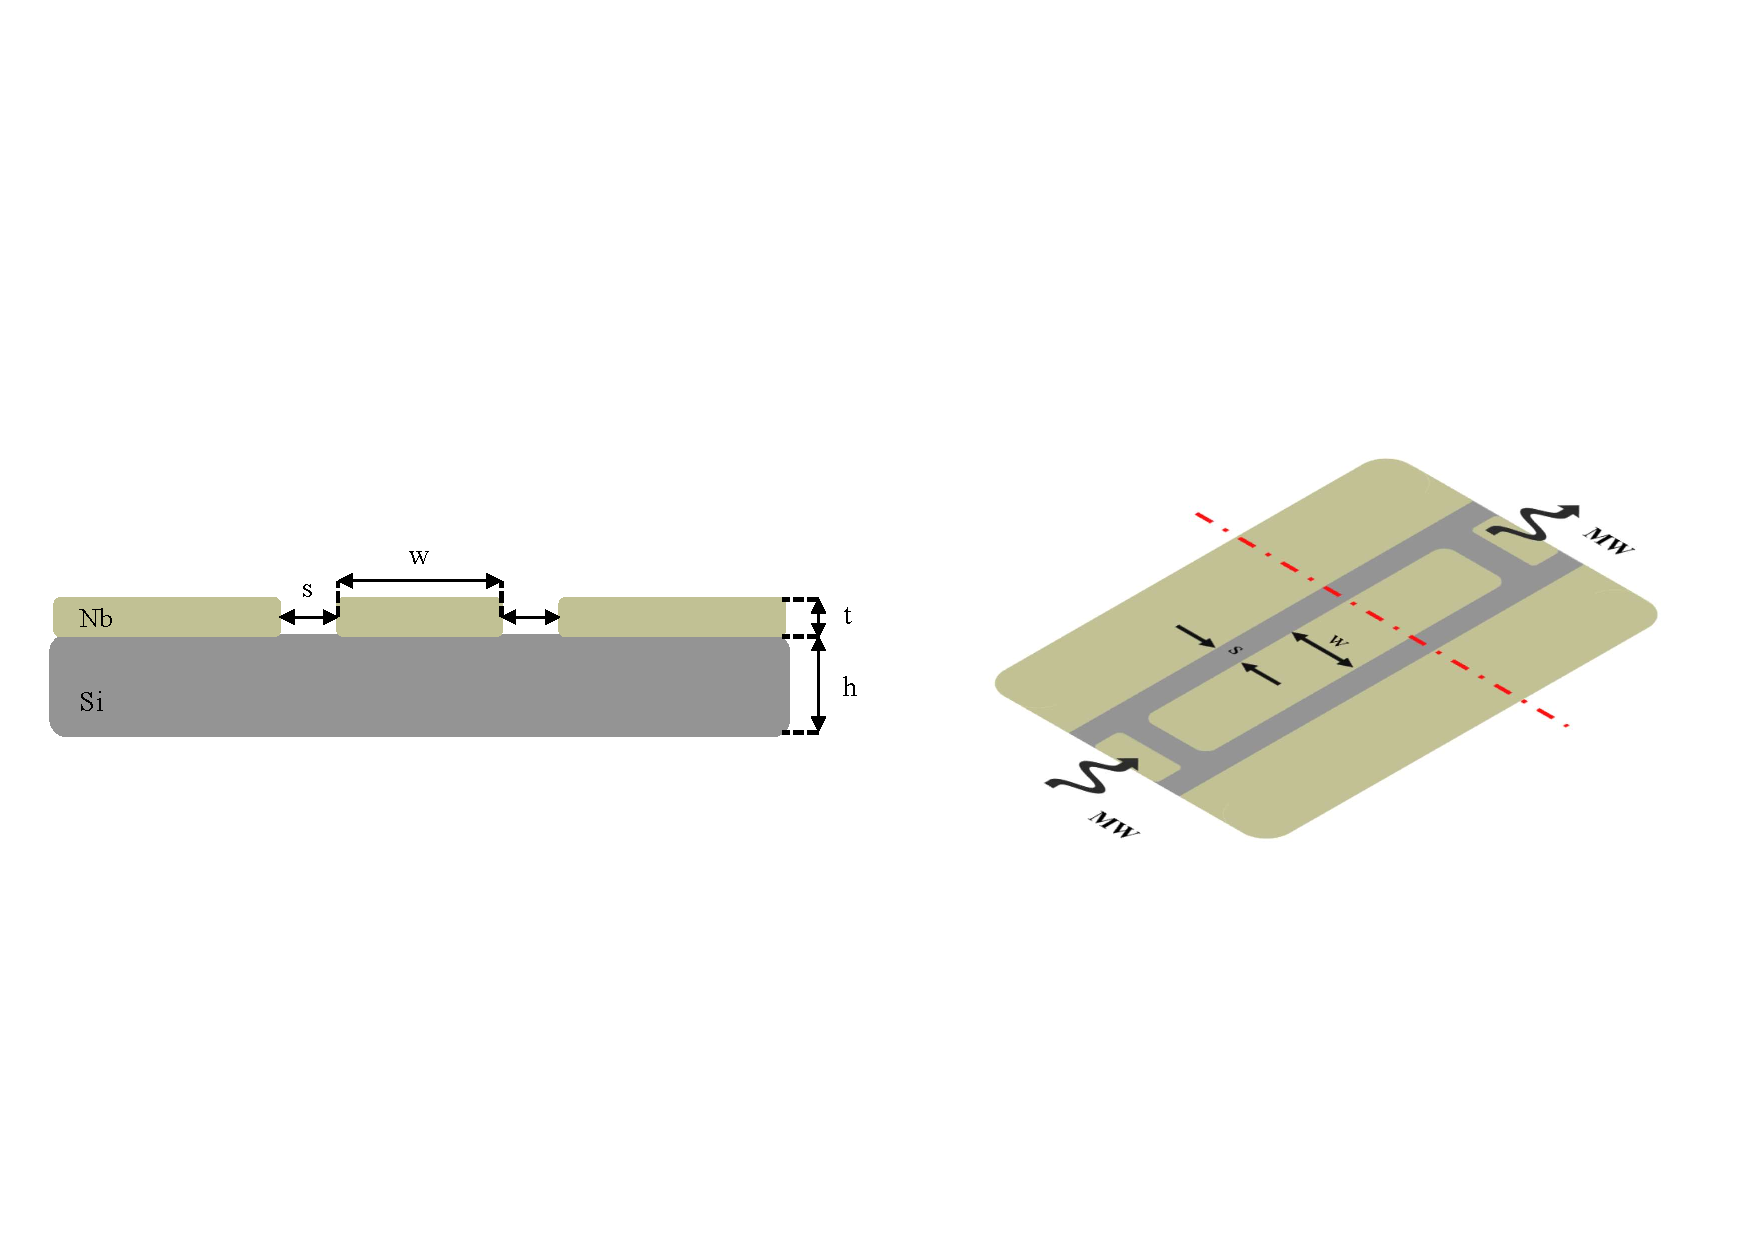
\includegraphics[width=14cm]{cpw2.pdf}
                \caption{CPW型断面図}
            \end{figure}
            CPW型共振回路の外観及び断面図を示した。CPW型回路は図中に示されたパラメータを調節することで回路のインピーダンスを適切に設計することができる。比較的簡便に高いQ値を持った共振回路を作成することができるため、超伝導量子エレクトロニクスの分野では頻繁に利用されている。当研究室ではSiの誘電率$\epsilon_r=11.9$を設計パラメータとして$s=6,w=10,t=50nm,h=450nm$を使用している。
            \begin{figure}[H]
                \centering
                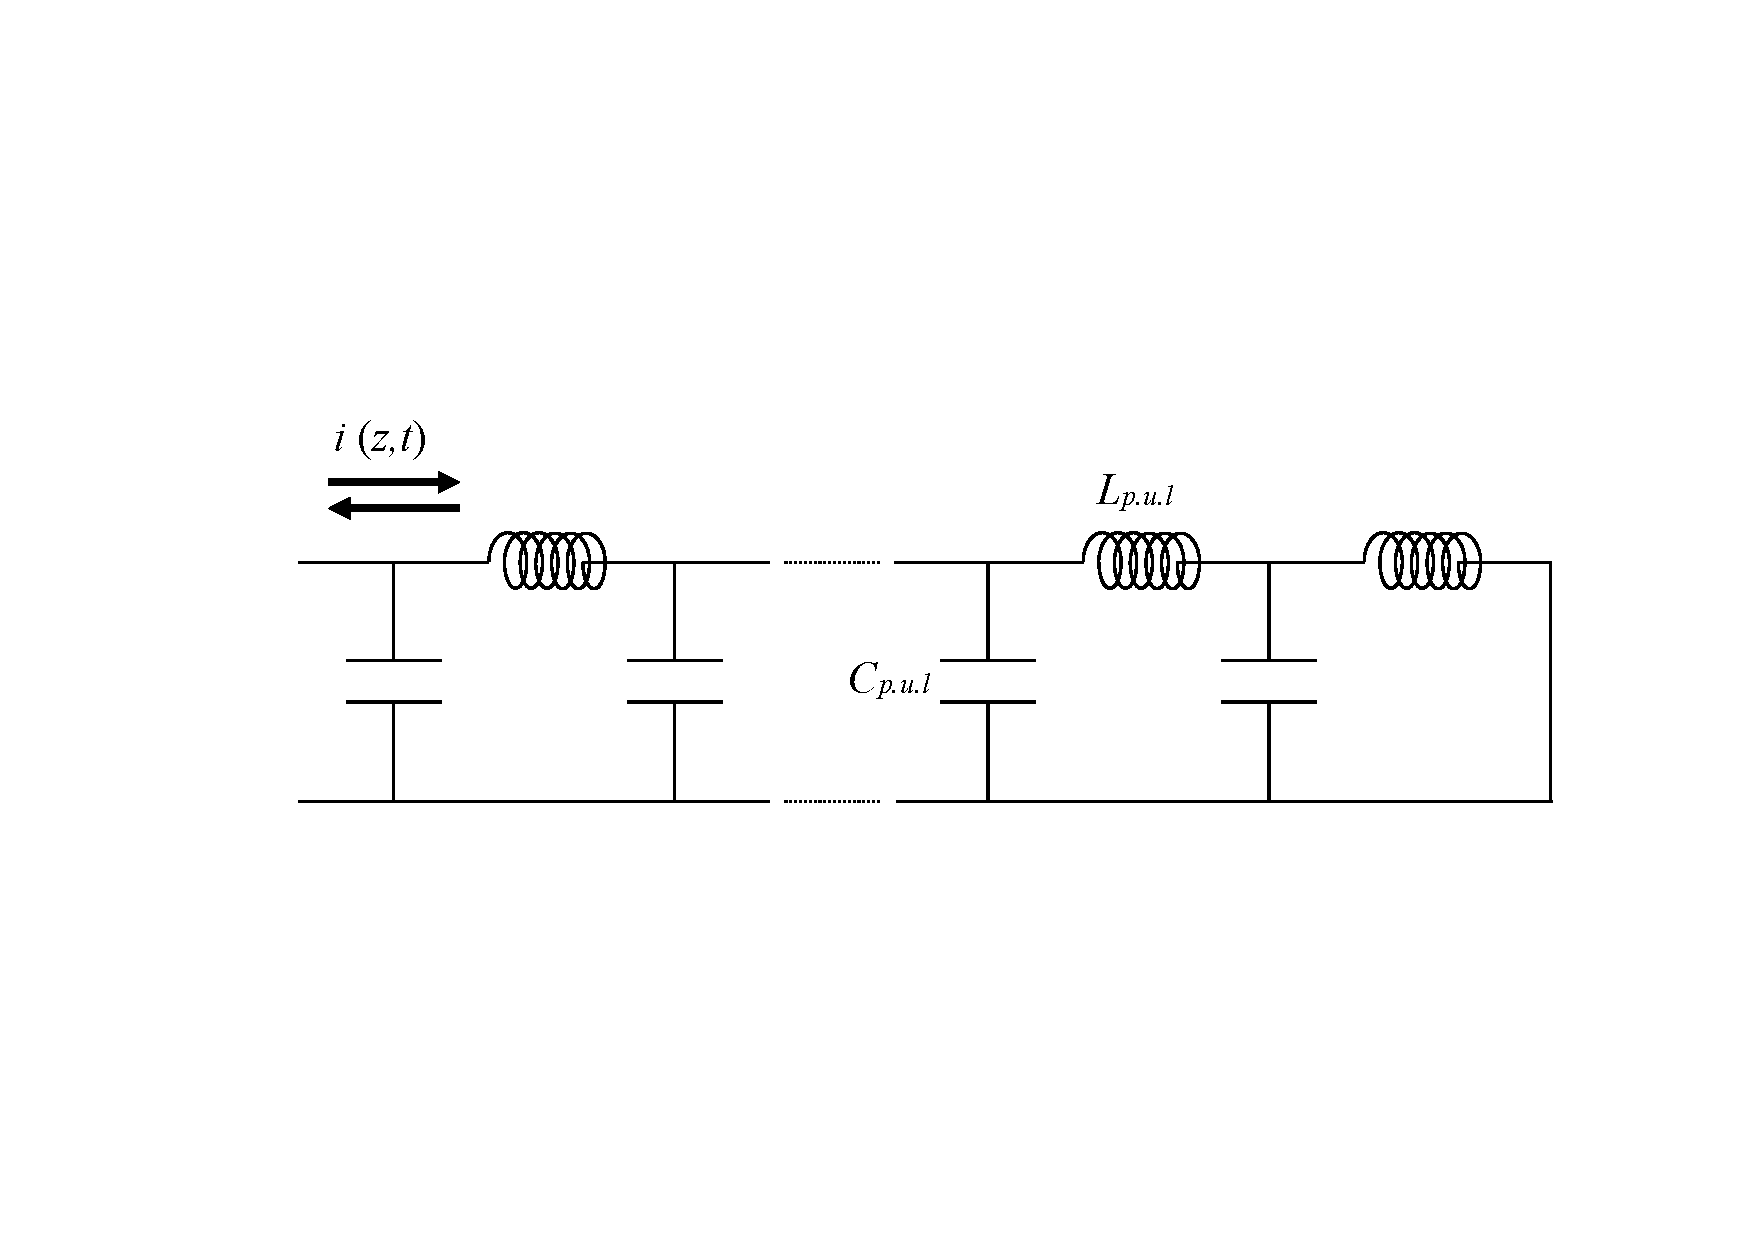
\includegraphics[width=9cm]{cpw.pdf}
                \caption{分布定数回路}
            \end{figure}
            分布定数回路は単位長さあたりのインピーダンスが一定に保たれているため、損失が少ない。単位長さあたりのキャパシタンスとインダクタンスをそれぞれ$C_l$、$L_l$とすると回路全体の共振周波数は
            \begin{equation}
                f_{0}=\frac{1}{2l\sqrt{L_l C_l}}
                \end{equation}
            と表記できる。ここで$2l=\lambda_0$である\cite*{Goppl2008,Besedin2018,inomata}。CPW型共振器において単位長さあたりのキャパシタンス及びインダクタンスはコンフォーマルマッピングという計算方法によって以下のように求めることが可能である。
            \begin{equation}
                L_{\ell}=\frac{\mu_{0}}{4} \frac{K\left(k_{0}^{\prime}\right)}{K\left(k_{0}\right)}
            \end{equation}
            \begin{equation}
                C_{\ell}=4 \epsilon_{0} \epsilon_{\mathrm{eff}} \frac{K\left(k_{0}\right)}{K\left(k_{0}^{\prime}\right)}
            \end{equation}
            \begin{equation}
                \begin{array}{l}
                k_{0}=\frac{w}{w+2 s} \\
                k_{0}^{\prime}=\sqrt{1-k_{0}^{2}}
                \end{array}
            \end{equation}
            ここでKは第一種楕円積分を表している。実際には超伝導体を用いているため、単位長さあたりのカイネティックインダクタンスも考慮しなければならない。サンプルの設計においては上記幾何学構造に依存するキャパシタンス及びインダクタンスを求めた後、カイネティックインダクタンスを別途求める必要があることに注意が必要である。すなわち
            \begin{equation}
                L(t, T)=L_{g}(t)+L_{k}(t, T)
            \end{equation}
            ここで前項が幾何学的構造に依存するインダクタンス、2項目がカイネティックインダクタンスである。カイネティックインダクタンスについてはさらに
            \begin{equation}
                L_{k}=\frac{\mu_{0}}{\pi^{2}}(\lambda / w) \ln (4 w / t) \frac{\sinh (t / \lambda)}{\cosh (t / \lambda)-1}
            \end{equation}
            と表現することができる。ここで$\mu_0$は真空の透磁率であり、$\lambda_0$は超伝導体薄膜に置ける磁場侵入長である。磁場侵入長$\lambda_0$は超伝導体の転移温度に於ける超伝導エネルギーギャップに依存するため、物質固有の値である。続いて超伝導準集中定数共振回路について解説する。
        \subsubsection{超伝導準集中定数回路}
            超伝導準集中定数回路は局所的に大きなキャパシタンスとインダクタンスを設けることでLC共振を実現している。回路デザインは下記のようにミアンダインダクタンスとインターデジタルキャパシタと呼ばれる幾何学的構造を作ることでキャパシタンスとインダクタンスを別々に作り出すという方法が一般的である。
        \begin{figure}[H]
            \centering
            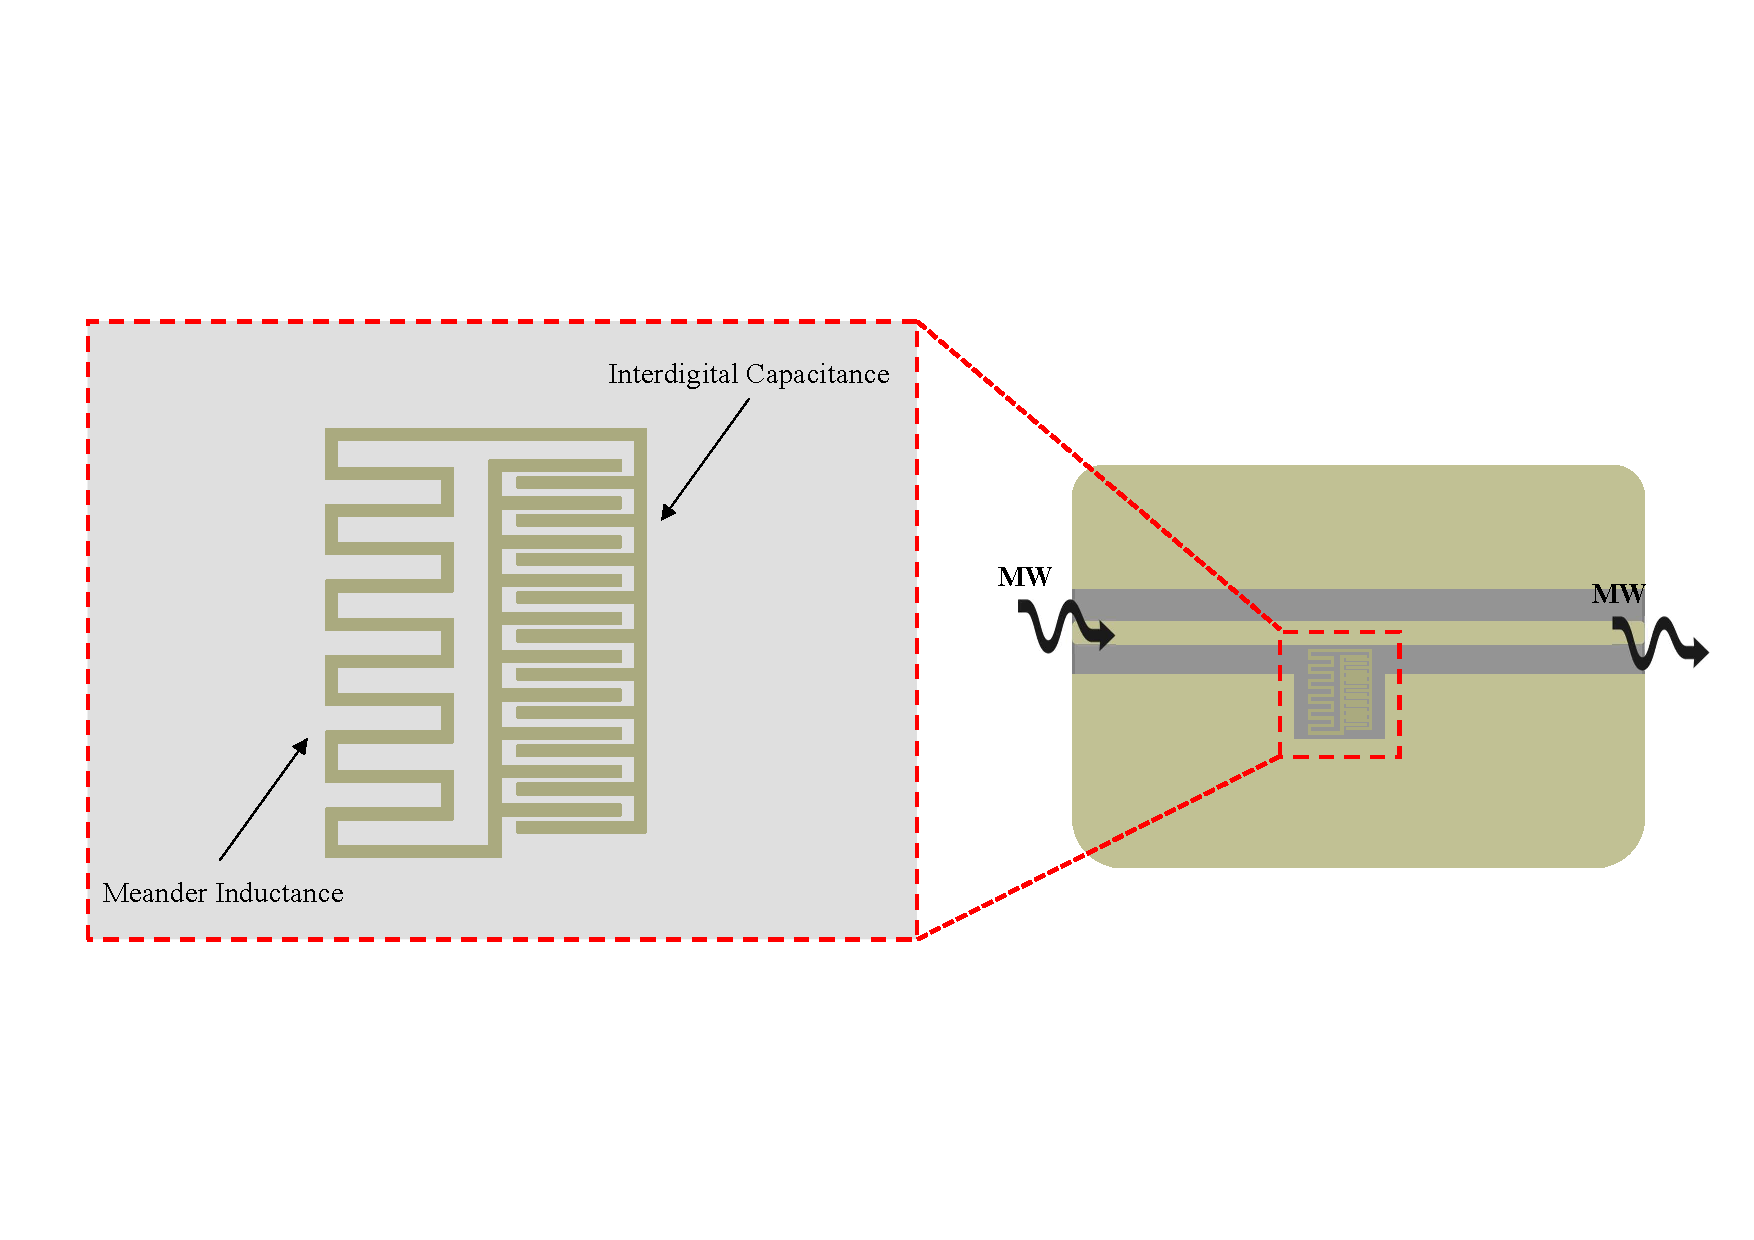
\includegraphics[width=14cm]{lumpedelement.pdf}
            \caption{超伝導準集中定数回路}
        \end{figure}
            \begin{figure}[H]
                \centering
                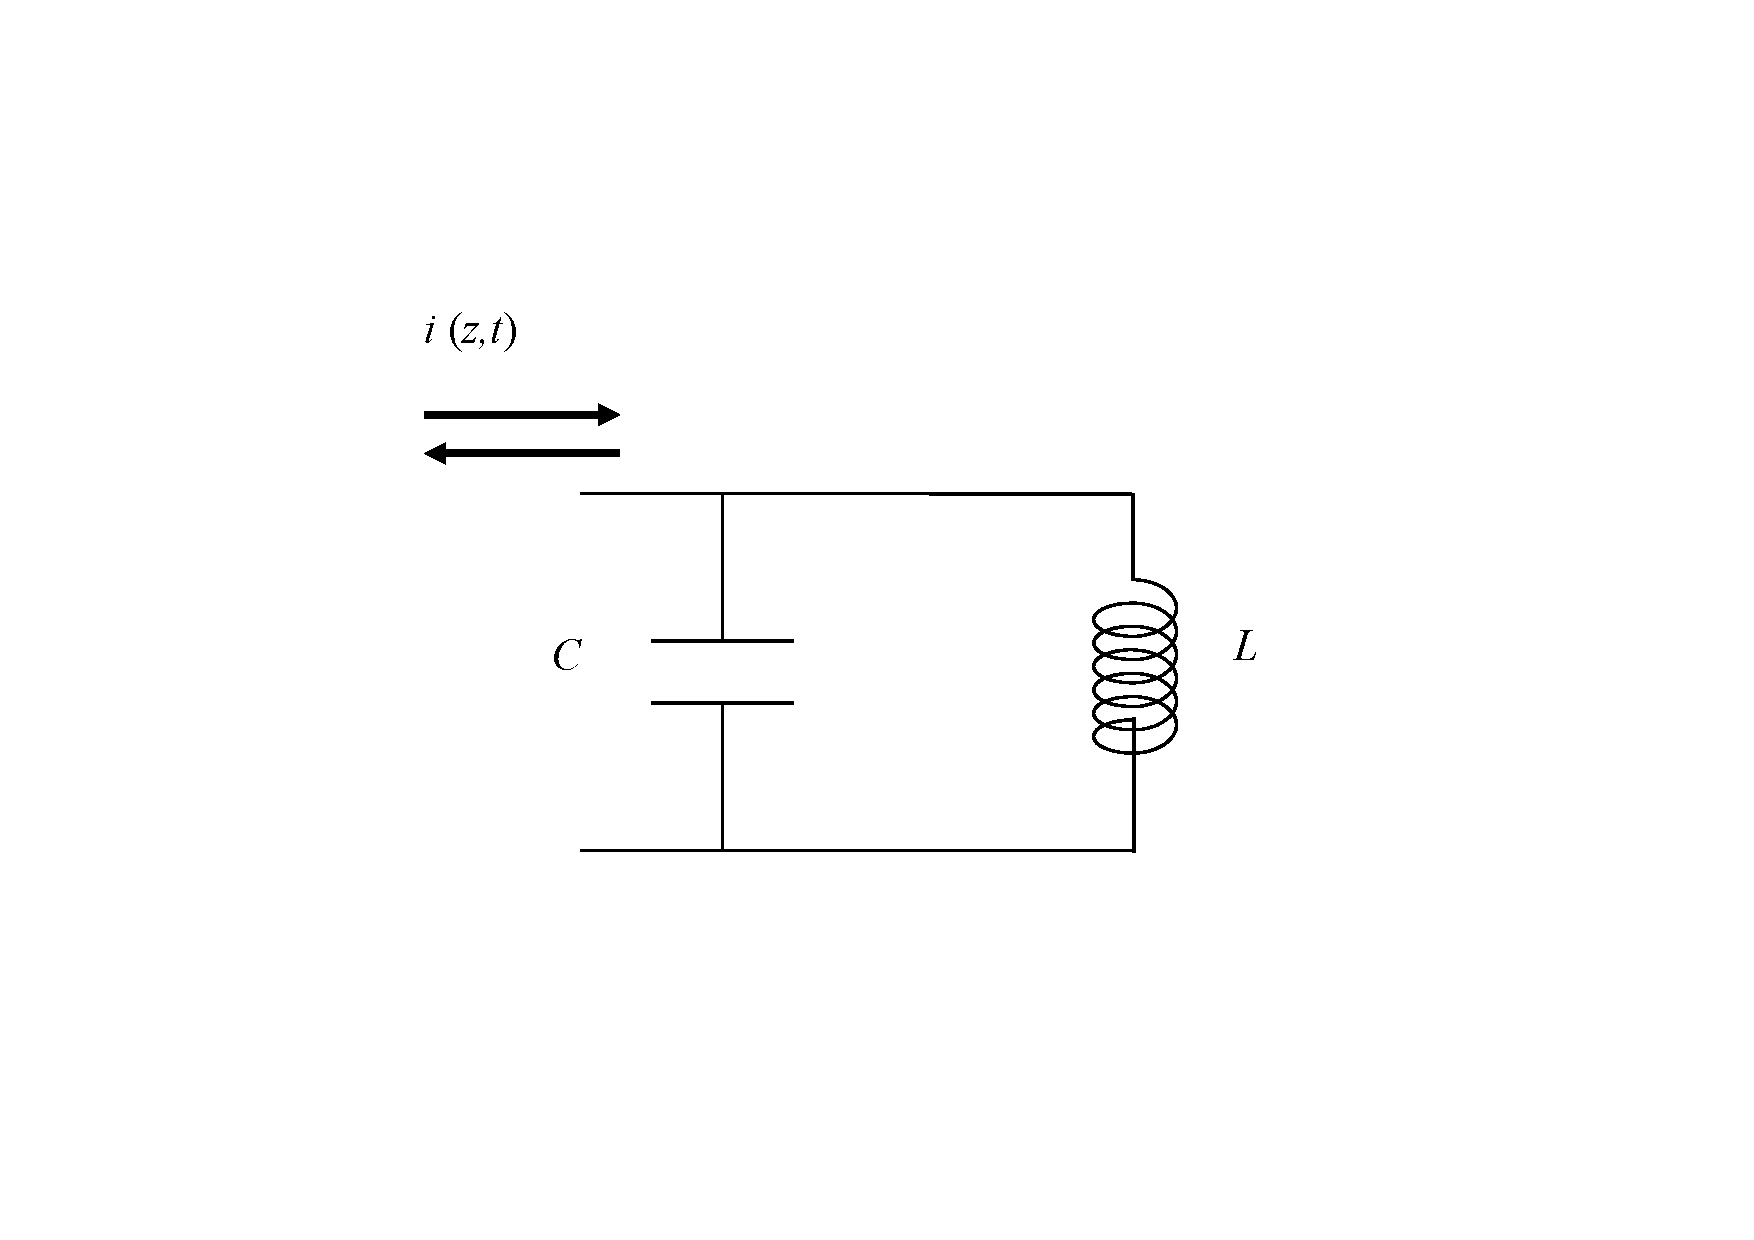
\includegraphics[width=9cm]{le.pdf}
                \caption{エネルギースペクトル}
            \end{figure}
            インターデジタルキャパシタンス及びミアンダインダクタンスの詳細な計算方法については付録に記載する。
    \subsection{ジョセフソン接合}
            ここまで超伝導共振器について解説してきた。ここでは超電導量子エレクトロニクスにおいて最も重要な素子、ジョセフソン接合について記述する。
            ジョセフソン接合は量子ビットやJPA(ジョセフソンパラメトリック増幅器)や結合素子等、超伝導共振素子と同じく幅広く利用されている素子である。
            量子ビットを作る際においてはジョセフソン接合がもたらす非調和性により、擬似的に2準位原子を作り出すことを可能にしている。本稿の的テーマである結合素子においてもジョセフソン接合が非常に重要な素子となる。本稿においてはrf-SQUID及びdc-SQUIDを構成する素子としてジョセフソン接合を導入するが、それぞれの素子の説明を行う前にジョセフソン接合の基本的な原理をこの章で説明する。
            \begin{figure}[H]
                \centering
                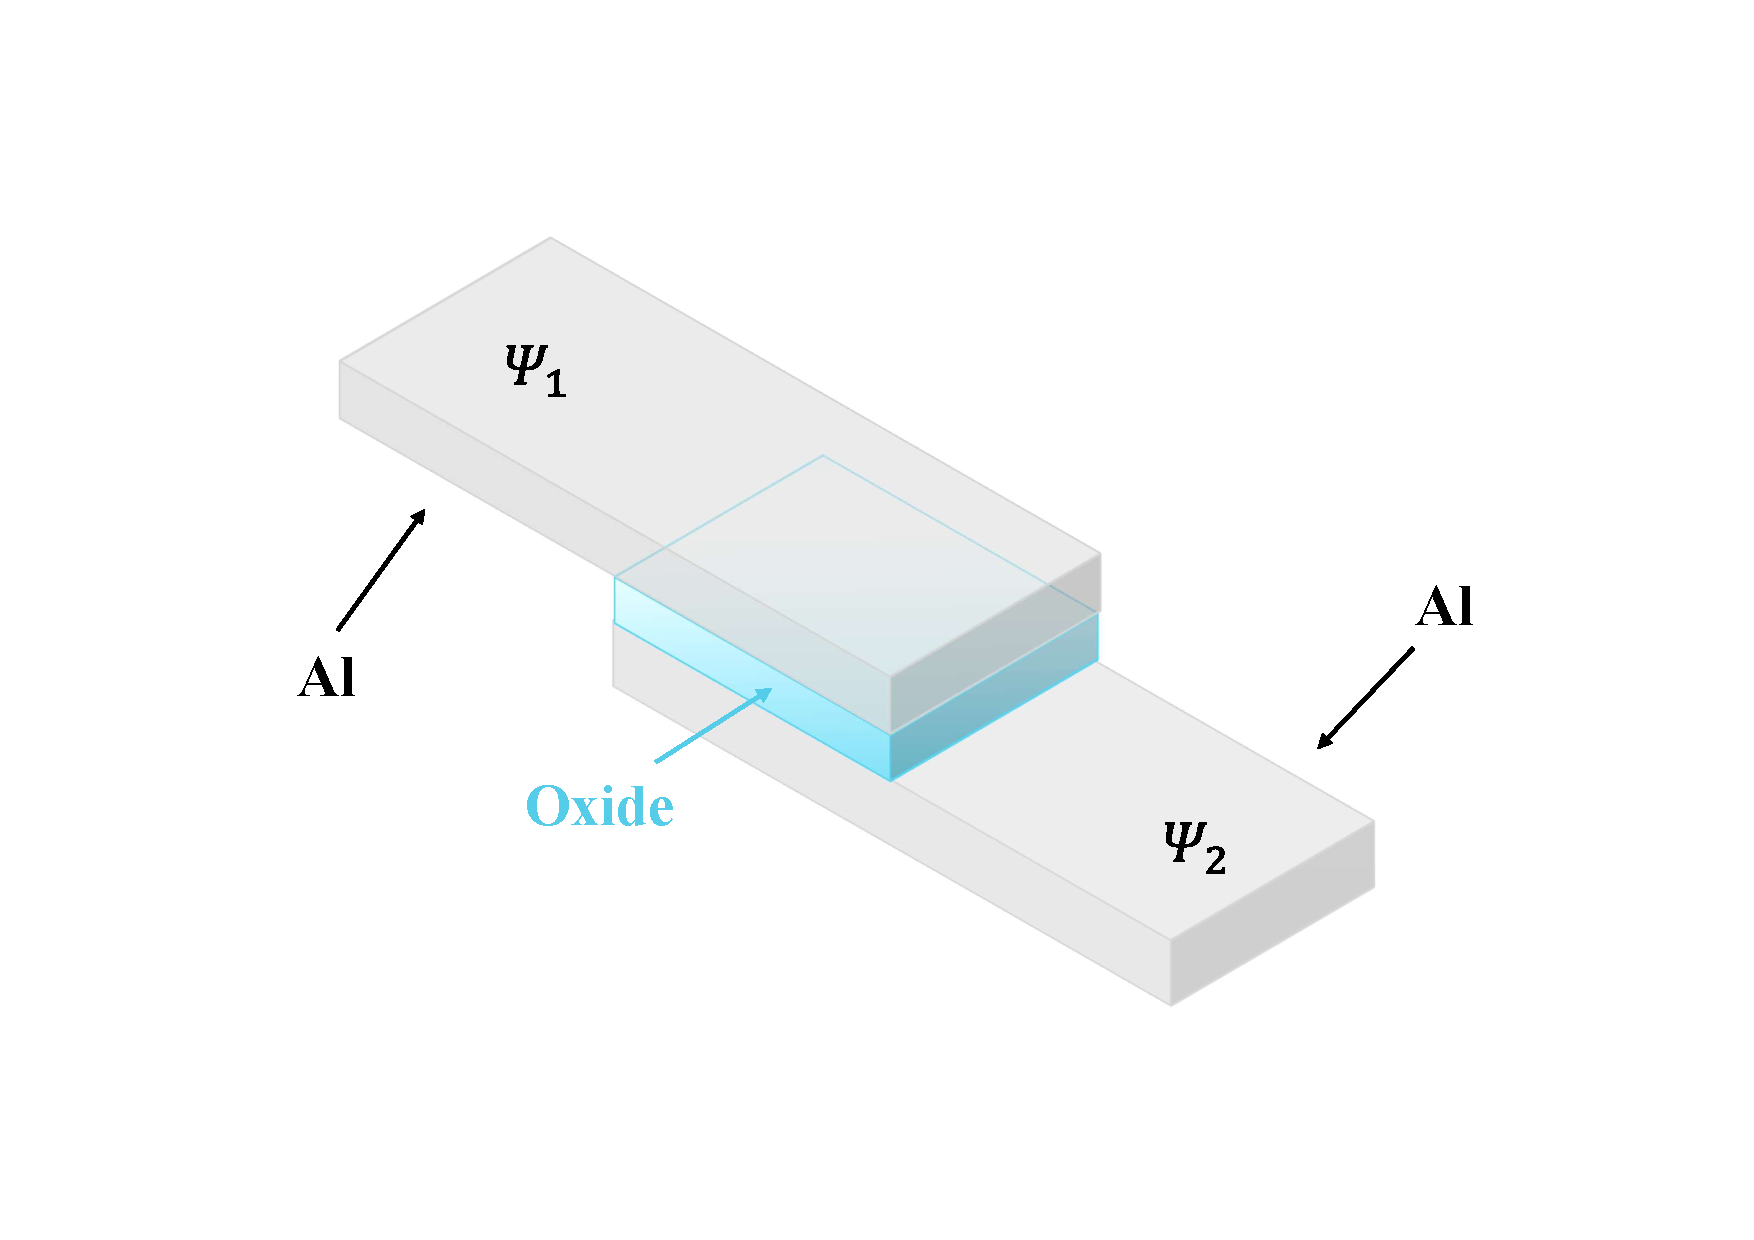
\includegraphics[width=9cm]{jj.pdf}
                \caption{ジョセフソン接合}
            \end{figure}
            ジョセフソン接合の形成方法はいくつかあるが、当研究室で採用している方法はSIS(超伝導体-絶縁体-超伝導体)型である。
            超伝導体間にアルミナ(Al2O3)を挟むことでジョセフソン接合を形成している
            ここではjosephson接合による物理的効果を理論から解説していくこととする。
            \begin{figure}[H]
                \begin{minipage}[t]{0.5\columnwidth}
                    \centering
                    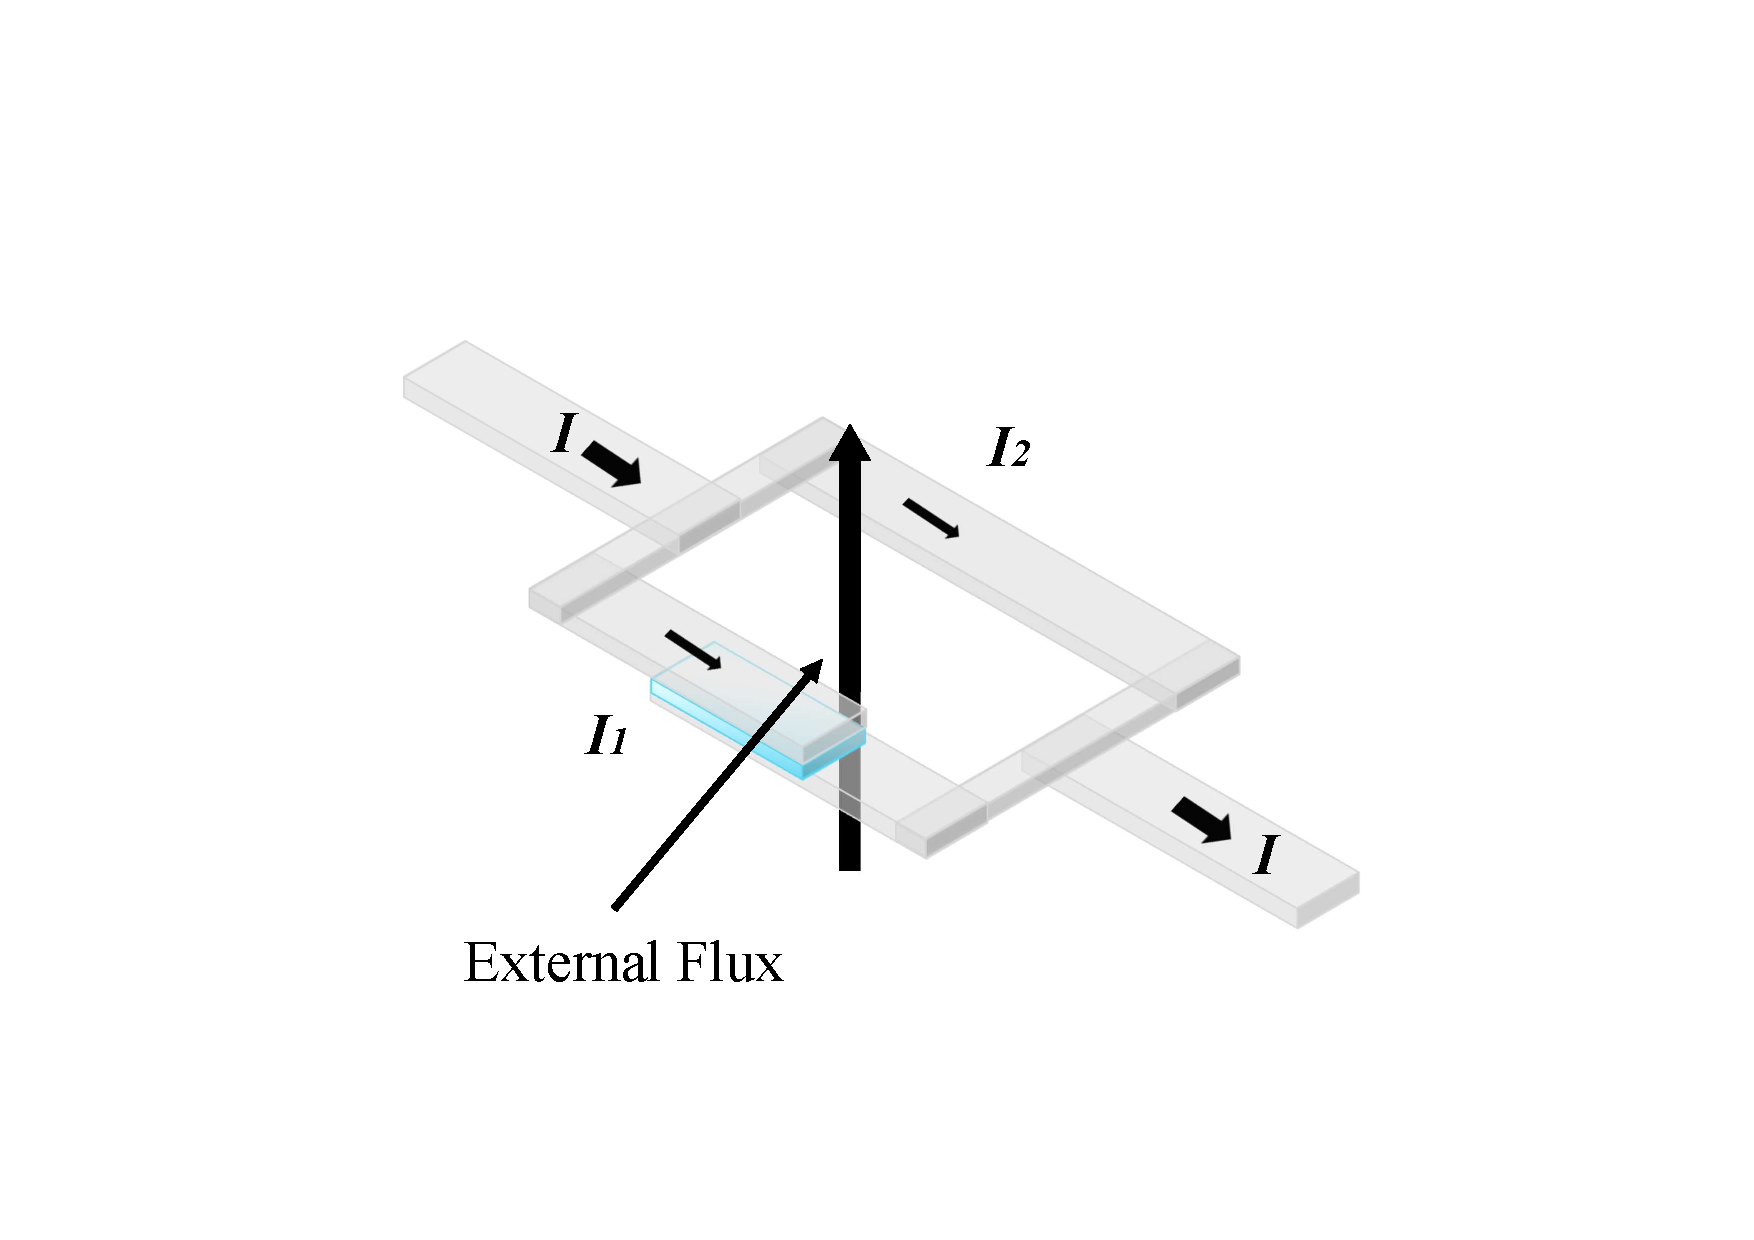
\includegraphics[clip, width=1.0\columnwidth]{rfsquid.pdf}
                    \caption{rf-SQUID}
                \end{minipage}%
                \begin{minipage}[t]{0.5\columnwidth}
                    \centering
                    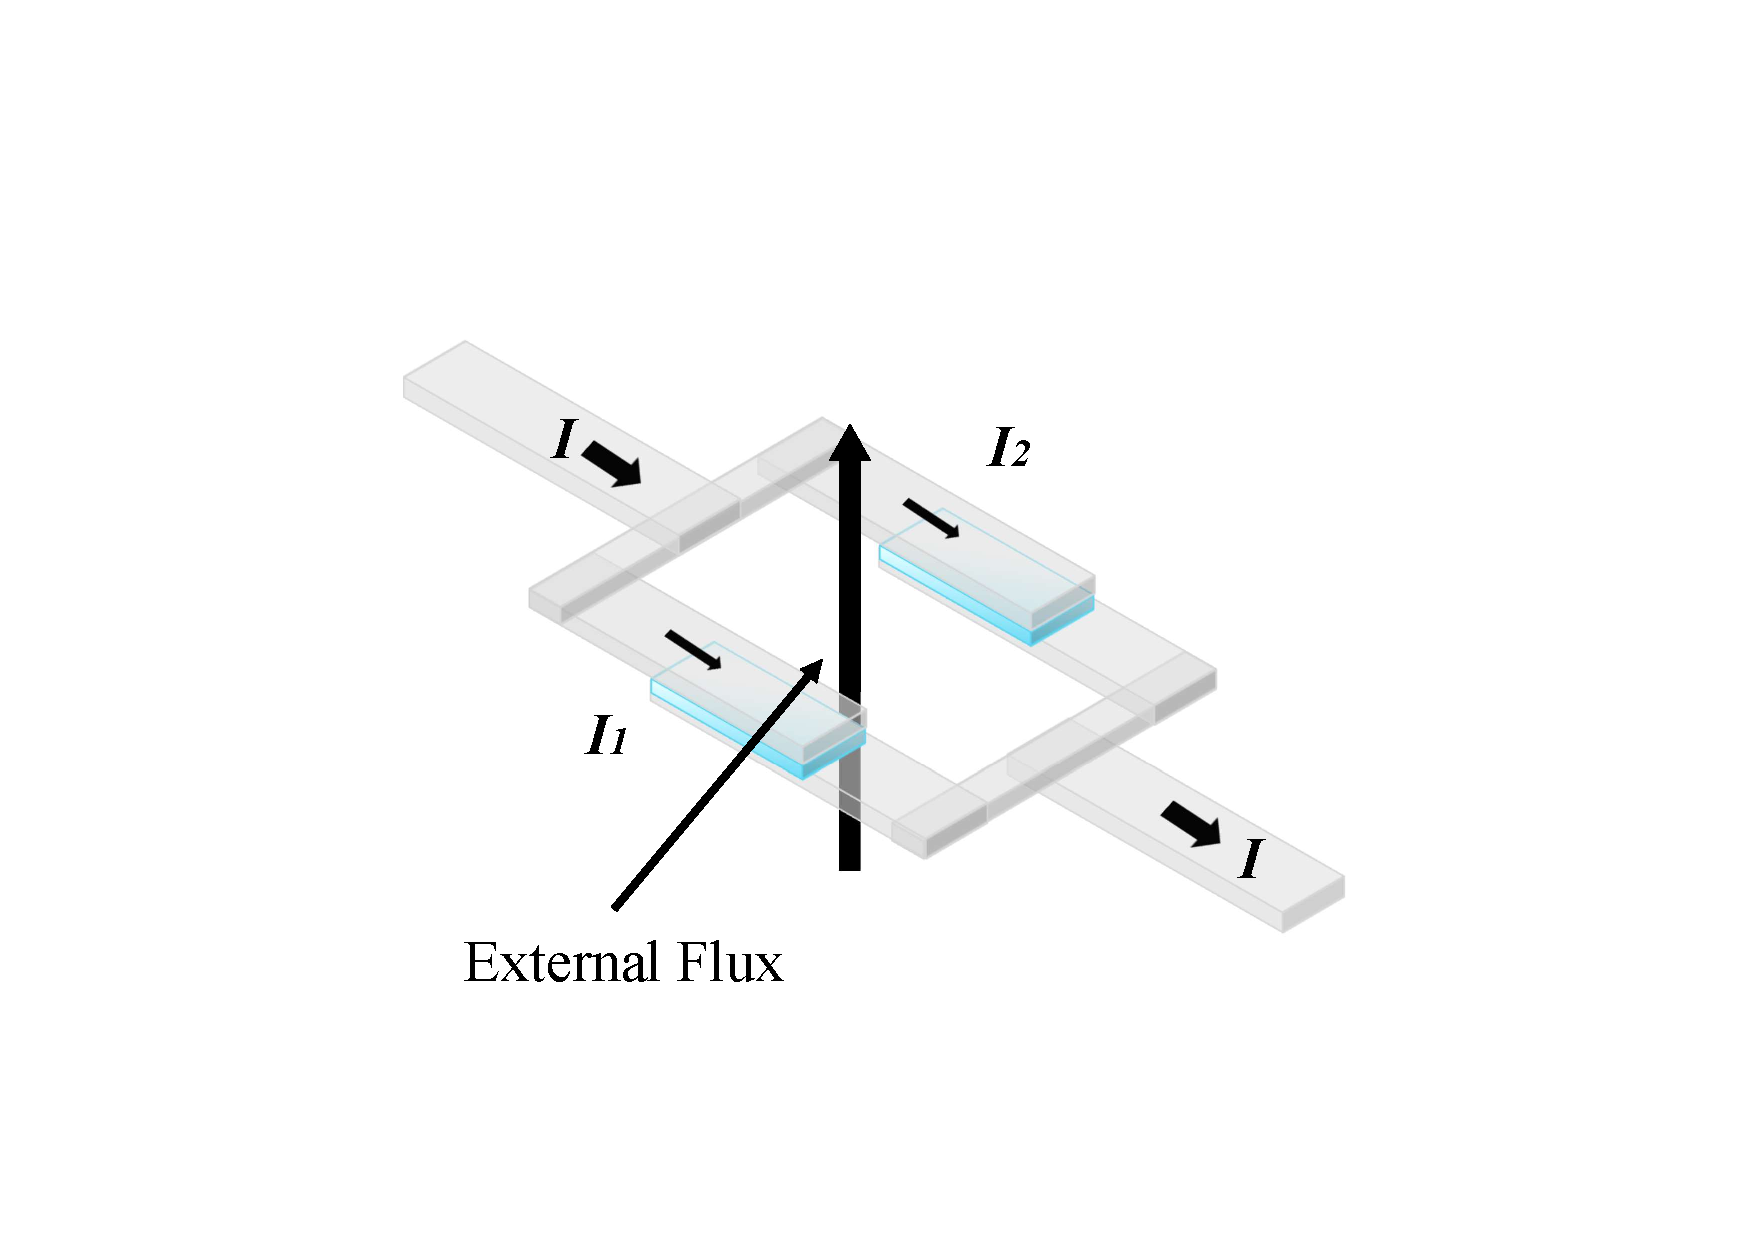
\includegraphics[clip, width=1.0\columnwidth]{dcsquid.pdf}
                    \caption{dc-SQUID}
                \end{minipage}
            \end{figure}

            この接合により生じsる物理的現象を、発見者の名に因んでjosephson効果と呼ぶ。
            この現象は大別するとACjosephson効果、DCjosephson効果の2つに分けることができる。
            この2つの効果についてGL理論から解説を始めることとする。
            \subsubsection{dc josephson効果}
                josephsonが1962年に行った理論的予言によれば、2つの超伝導体の間にゼロ電圧下で以下のような超伝導電流が流れるとしている。
                \begin{equation*}
                    I_s = I_c \sin(\Delta \psi)
                \end{equation*}
                ここで$\Delta \psi$とはGL波動関数のs位相差である。:また、臨界電流$I_c$は接合に流すことのできる、最大の超伝導電流である。
                彼はさらに接合に電位差vが生じているときに位相差が次のように振動すると予言した。
                \begin{equation*}
                    \frac{d(\Delta \psi)}{dt} = \frac{2eV}{\hbar}
                \end{equation*}
                これにより、電流は振幅を臨界電流$I_c$、周波数を$\nu = \frac{2eV}{h}$の交流となる。
                つまり、この電流変化はエネルギー$h\nu$でクーパー対が接合を通過するエネルギーと一致していることがわかる。
                以上2つの関係式によりこの接合により蓄えられるエネルギーは
                \begin{eqnarray}
                    \int_0^{t} (I_s V)dt&=&\int_{0}^{\delta} I_s(\hbar/2e)d\delta\\
                    &=&E_j(1-\cos(\delta))\\
                \end{eqnarray}
                と表現することができる。ここで$E_j=\hbar I_c/2e$である。
    \subsection{rf-SQUID}
                rf-SQUIDは
    \subsection{dc-SQUID}
        dc-SQUIDは超伝導ループ両枝にジョセフソン接合を一つずつ導入したものである。磁束量子干渉計とも呼ばれ広範囲の分野で応用されている素子である。代表的な例を上げれば重力波の観測やなどに使われている。外部磁場に非常に敏感であり
        dc-SQUIDを導入する意図はrf-SQUIDのジョセフソン接合を可変にするためである。これによりrf-SQUIDのジョセフソンインダクタンスは外部磁場に対し変化する。
        \begin{figure}[H]
            \centering
            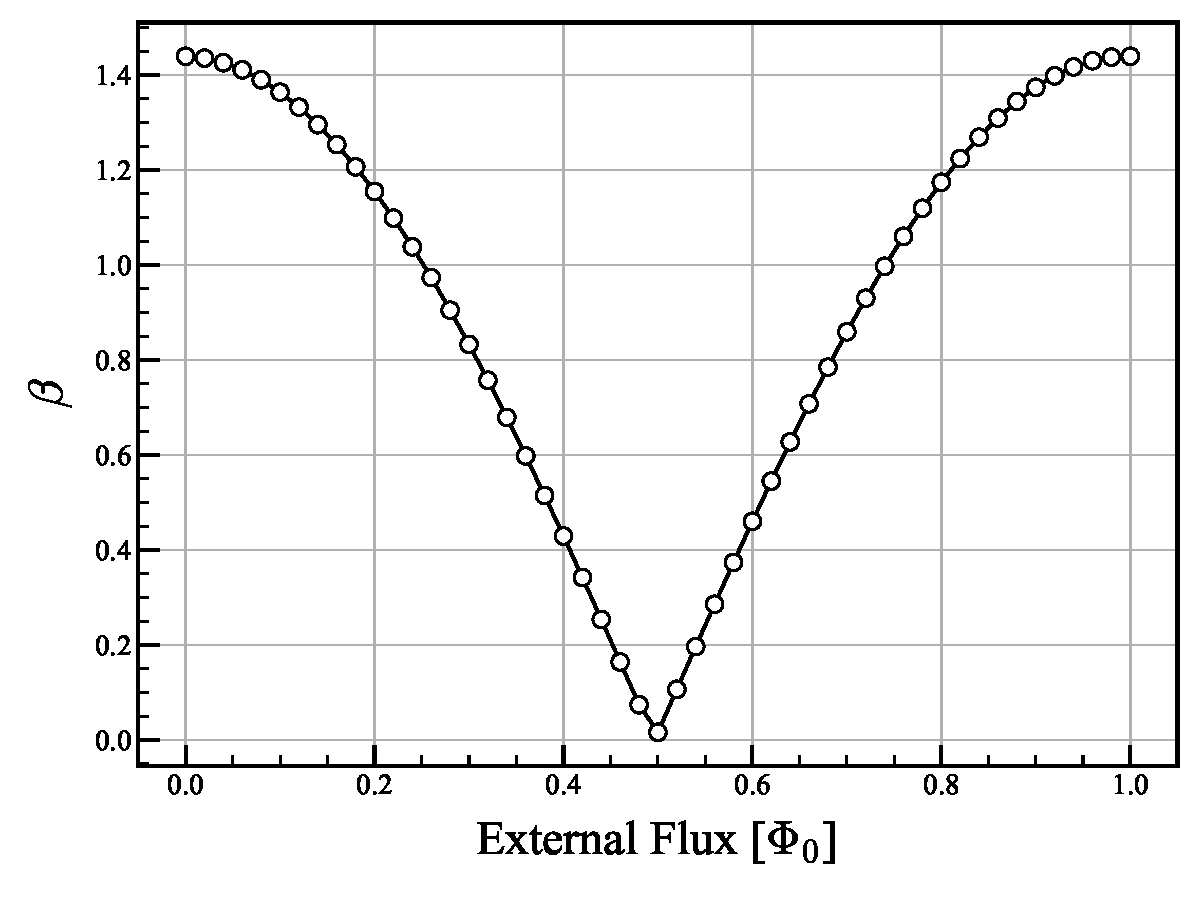
\includegraphics[width=9cm]{dc-squid.pdf}
            \caption{エネルギースペクトル}
        \end{figure}
        ではこのdc-SQUIDによってどのようジョセフソンインダクタンスが変化するのかを示す。
    \subsection{カイネティックインダクタンス}
        カイネティックインダクタンスは超伝導インダクタンスとも呼ばれる。超伝導細線を扱うとこのインダクタンスの影響が大きくなる。超伝導体中の準粒子移動により誘導されるインダクタンスである。このカイネティックインダクタンスは物質固有の値であり、非常に局所的な領域で大きなインダクタンスを得られるため、この特性を利用した量子ビットなども存在する。今回限られた設計内でおおきなインダクタンスを得るためにこのカイネティックインダクタンスを導入した。次節導入するミアンダインダクタンスは1μで加工されており、カイネティックインダクタンスの影響が大きく現れるとよそうされる。
    \subsection{ミアンダインダクタンス}
        ミアンダとは蛇行したという意味である。図の通り単純な直線ラインではなく折り返し構造を繰り返すことで、実質的な長さ、ライン間の相互インダクタンスにより総合的な自己インダクタンスが大きくなる。このミアンダインダクタンスを導入する上で論文の解析を利用した。計算方法を補足に記したので参照されたい。計算結果のみを示すと下図の構造に与えられた数値を入力することで得たいインダクタンスを求めることが可能である。次章でも言及するがこのミアンダインダクタンスの数値を考える上でもう一つ電磁界シミュレーションによる方法もとったのでここで紹介する。
        電磁界シミュレーションにはnational instruments社のマイクロウェーブオフィスを利用している。CADファイルで設定されたオブジェクトに材質特性を付与し電磁波の入出ポートを設定することで反射特性等を計算することが可能である。
        ここでシミュレーションする構造物は下図のようなミアンダインダクタンスのない単体の共振器とミアンダインダクタンスを導入した単体の共振器である。この2つのこの構造物全体のアドミッタンスを低周波数領域で計算することで構造物全体の伝導伝導性を計算することができる。アドミッタンス値からおおよその構造物のインダクタンスを計算することができるが2つの構造物の差分はおおよそミアンダインダクタンスの可否に依存する。そこでミアンダの数に対してインダクタンスがどれだけ増加するかプロットしたものが図である。この図からはミアンダの数に依存して線形にインダクタンスが増加していることがわかる。ここで上述した解析計算とどれだけの差があるかも同時にい示す。

        プロットの結果では0-100の範囲内で両者の乖離はおよそOOであった。さほど乖離はないといえるが参考値程度にとどめておく。今回のサンプル作成ではN=38をミアンダインダクタンスとして採用した。
        
        